
We have shown in section \ref{section:selection} that we can reject background triggers using selection criteria based on the excess rate and gating.
In the same section we also considered a cut on the $\achi$ to reduce the background.
This cut turned out to unsafe.
This is explained by the fact that for injections, and therefore astrophysical signals, the $\achi$ grows with the SNR.
Therefore, removing high $\achi$ events at high SNR will remove both noise and astrophysical triggers.

In this chapter we will study this dependency of the $\achi$.
The goal would be to find a way to improve the $\achi$ or the rwSNR such that very loud astrophysical signal and injections are not downgraded by them.
This study is not conclusive, therefore the purpose of this section is to document it in order to highlight the challenges and what might be done in the future.


%%%%%%%%%%%%%%%%%%
\label{sec:improve_achi2}

The rwSNR (eq. \ref{eq:rwsnr}) was introduced to downrank background candidates relative to astrophysical events.
It is based on the computation of the $\achi$ (eq. \ref{eq:achi2})  which computes, upon detection of a candidate, the excess of power due to mismatch between the measured signal and the theoretical one, expected from the template that triggered.
The rwSNR proved to be very useful in background removal.
As already reminded, there is however a downside to the \achi: its value grows as the SNR grows.
This is especially visible when looking at simulated events (injections).
This is shown on figure \ref{fig:achi2_vs_snr} where we can see that almost no BBH injection with SNR greater than 30 keeps more than 80\% of its SNR after reweighting.
It also shows the rwSNR vs SNR distribution for those injections.
We clearly see that many loud injections end up with a much lower rwSNR.
This means that some loud injections and astrophysical events can be missed because their SNR is too heavily reweighted.

The origin of of higher \achi at high SNR is the discreet nature of the template bank.
It results in a small mismatch between the source and template parameters and thus in waveforms.
These small differences become significant for high SNR events.

In this chapter we only study L1 as it is the detector with the highest sensitivity and therefore the highest SNRs.
It makes a good case of the issues at hand.

\begin{figure}[ht]
    \centering
    \begin{minipage}{0.45\linewidth}
        \centering
        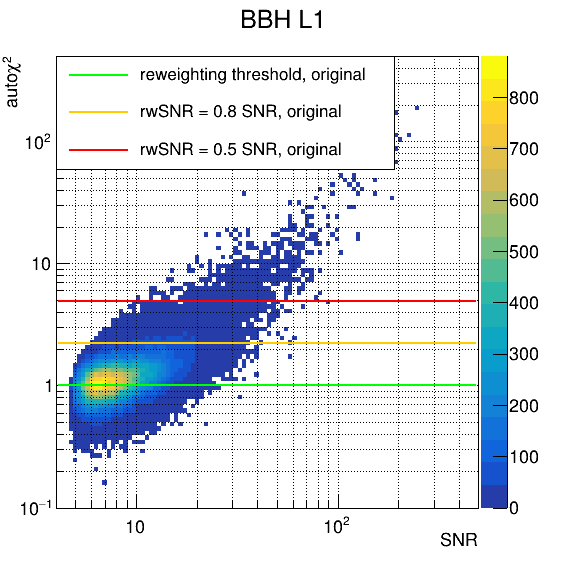
\includegraphics[width=\linewidth]{sectionImprovement/rwSNR/cSnrAchi2_L1.png}
    \end{minipage}
    \hfill
    %
    \begin{minipage}{0.45\linewidth}
        \centering
        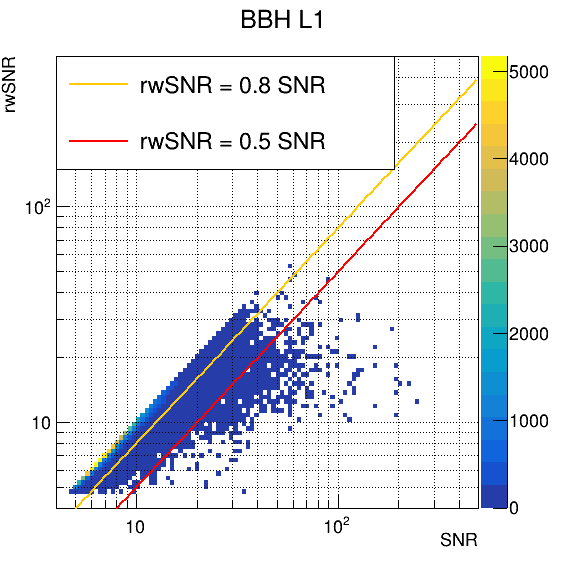
\includegraphics[width=\linewidth]{sectionImprovement/rwSNR/cSnrRw_L1.png}
    \end{minipage}
    \hfill
    \caption{O3 BBH recovered injections: \achi vs SNR (left) and rwSNR vs SNR (right) for single detector triggers associated to coincidences. Various rwSNR threshold are plotted using equation \ref{eq:rwsnr}.}
    \label{fig:achi2_vs_snr}
\end{figure}


%%%%%%%%%%%%%%%%%%%%%%%%%%%%%%%%%%%%%%%%%%%%%%%%%%%%%%%%%%%%%%%%%
%%%%%%%%%%%%%%%%%%%%%%%%%%%%%%%%%%%%%%%%%%%%%%%%%%%%%%%%%%%%%%%%%
%%%%%%%%%%%%%%%%%%%%%%%%%%%%%%%%%%%%%%%%%%%%%%%%%%%%%%%%%%%%%%%%%

\subsection{SNR dependency of the \texorpdfstring{\achi}{autoChi2}}
\label{sec:snr_dependency}

We want to parametrize the evolution of the \achi as a function of the SNR.
This would allow to take it into account in our reweighting to try to improve the rwSNR.
As mentionned earlier, it is caused by the discretization of the template bank.
The signal that we measure is in fact the theoretical signal to which we have to add the background and also the mismatch due to our discretized template bank.
The theoretical MFO is 
%
\begin{equation}
    \textrm{MFO}_{P/Q,exp}[i] = \textrm{SNR} \times \textrm{MFO}_{P/Q,exp,\text{normalized}}[i]
\end{equation}
%
The mismatch between the template and measured signal is therefore going to be proportional to the SNR.
If we go back to the expression of the \achi \ref{eq:achi2} and we write
%
\begin{equation}
\label{rewrite_mfo}
    \textrm{MFO}_{P/Q,meas}[i] = \textrm{MFO}_{P/Q,exp}[i] + \epsilon \textrm{SNR} + \textrm{bkg}
\end{equation}
%
where $\epsilon \textrm{SNR}$ is a term relative to the mismatch with the template proportional to the SNR and bkg is a background term of order 1, then we can write the \achi as follows:
%
\begin{align}
\label{eq:snr_dep}
    \achi &= \frac{1}{2\textrm{N}} \sum_{i=0}^{\textrm{N-1}} \left[  2(\epsilon\textrm{SNR}+bkg)^2 \right] = \epsilon^2 \textrm{SNR}^2 +2\epsilon\textrm{SNR$\times$bkg}+\textrm{bkg}^2\\
    \achi &\xrightarrow[\textrm{{\tiny large SNR}}]{} \epsilon^2\textrm{SNR}^2
\end{align}
%

Hence, we expect the \achi to grow with the SNR$^2$ at large SNRs.
We can now use the formula \ref{eq:snr_dep} to parameterize the \achi as a function of the SNR. 
Figure \ref{fig:fit_profile} shows the profile histograms of the \achi vs SNR graphs (like figure \ref{fig:achi2_vs_snr} for BBH) for the BBH, BNS and NSBH injections.
The profiles are fitted with
%
\begin{equation}
\label{eq:fit}
    \achi = \left(p_0 + p_1 \textrm{SNR} \right)^2
\end{equation}
%
We retrieve a value of order 1 for $p_0 = C$ as expected for the background term, and close to 3\% for $p_1 = \epsilon$ which is of the order of magnitude for the minimal match of the template bank.
%


% \begin{table}
% \centering
%     \begin{minipage}{0.45\linewidth}\centering
%         \begin{tabular}{c|c|c|c}
%                            & H1    & L1    & V1     \\\hline
%             $\chi^2$ / NDF & 8.45  & 9.96  & 7.56   \\\hline
%             $p_0$          & 0.83  & 0.82  & 0.80   \\\hline
%             $p_1$          & 0.031 & 0.031 & 0.037  \\
%         \end{tabular}
%         \caption{BBH injections: Results of the fit performed on the \achi vs SNR profile histograms.}
%         \label{tab:fit_results_bbh}
%     \end{minipage}
%     \hfill
%     %%
%     %%
%     \begin{minipage}{0.45\linewidth}\centering
%         \begin{tabular}{c|c|c|c}
%                            & H1    & L1    & V1     \\\hline
%             $\chi^2$ / NDF & 7.77  & 11.20  & 4.90   \\\hline
%             $p_0$          & 0.87  & 0.83   & 0.80   \\\hline
%             $p_1$          & 0.023 & 0.029  & 0.037  \\
%         \end{tabular}
%         \caption{BNS injections: Results of the fit performed on the \achi vs SNR profile histograms.}
%         \label{tab:fit_results_bns}
%     \end{minipage}
%     \hfill
%     %%
%     %%
%     \vspace{5mm}
%     \begin{minipage}{0.45\linewidth}\centering
%         \begin{tabular}{c|c|c|c}
%                            & H1    & L1    & V1     \\\hline
%             $\chi^2$ / NDF & 4.19  & 5.50  & 9.75   \\\hline
%             $p_0$          & 0.83  & 0.80  & 0.89   \\\hline
%             $p_1$          & 0.031 & 0.036 & 0.041  \\
%         \end{tabular}
%         \caption{NSBH injection: Results of the fit performed on the \achi vs SNR profile histograms.}
%         \label{tab:fit_results_nsbh}
%     \end{minipage}%
% \end{table}



\begin{figure}
  \centering
  \begin{minipage}{\linewidth}
    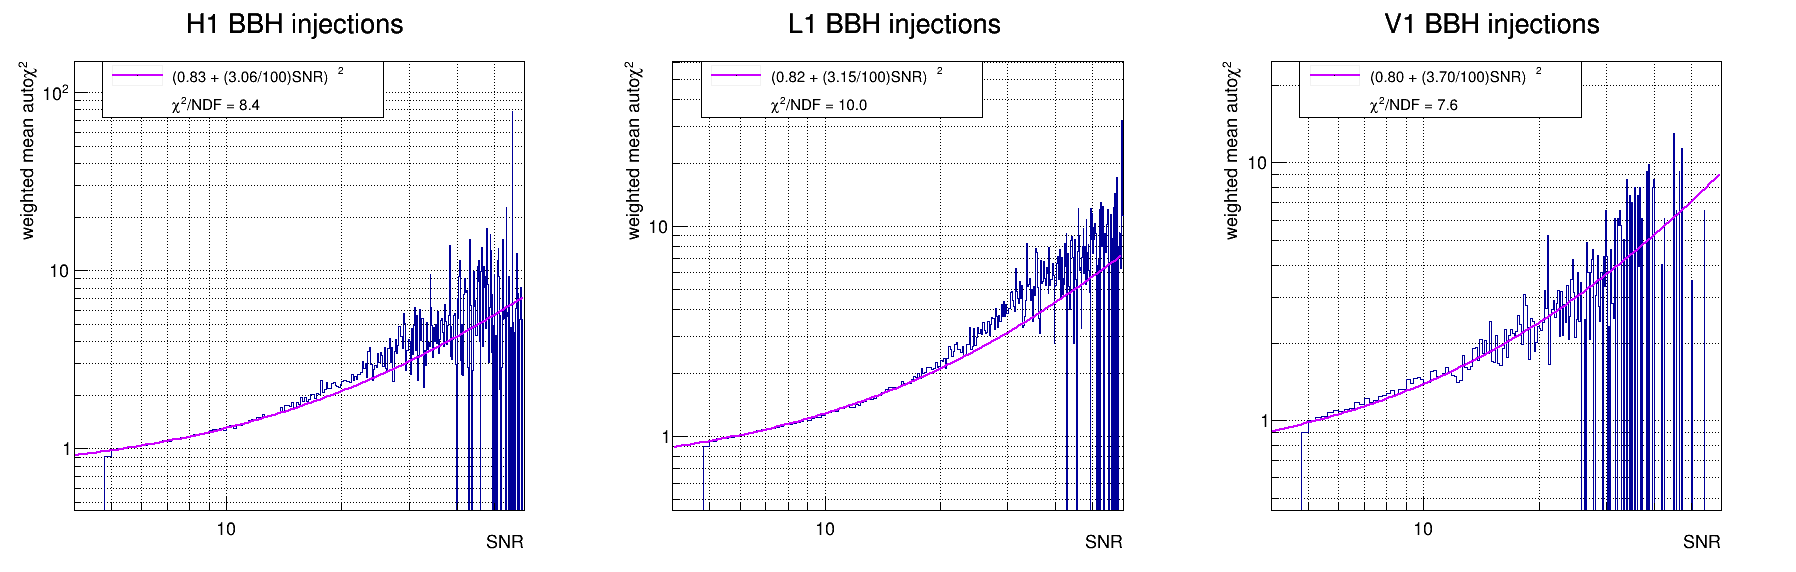
\includegraphics[width = \textwidth]{sectionImprovement/rwSNR/cProfile_BBH.png}
  \end{minipage}
  %% 
  \begin{minipage}{\linewidth}
    \centering
    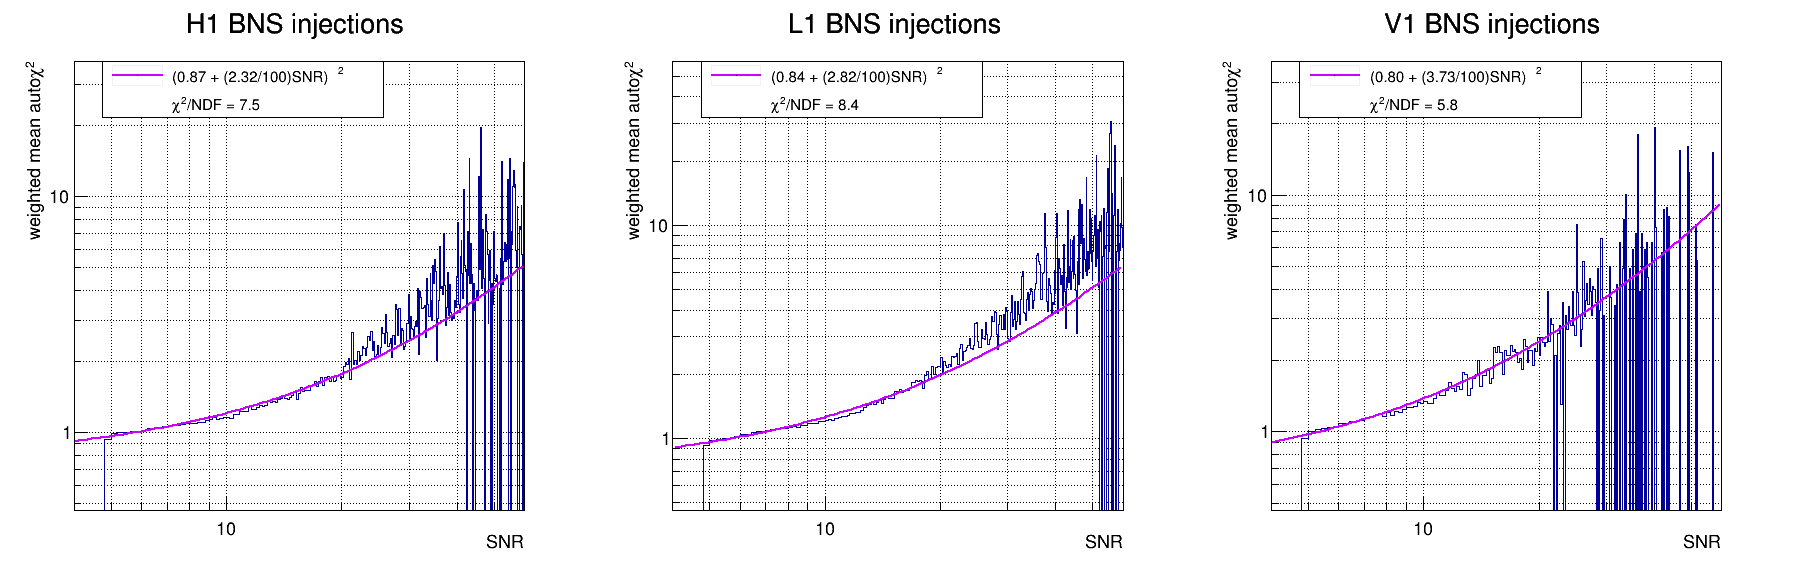
\includegraphics[width = \textwidth]{sectionImprovement/rwSNR/cProfile_BNS.png}
  \end{minipage}
  %% 
  \begin{minipage}{\linewidth}
    \centering
    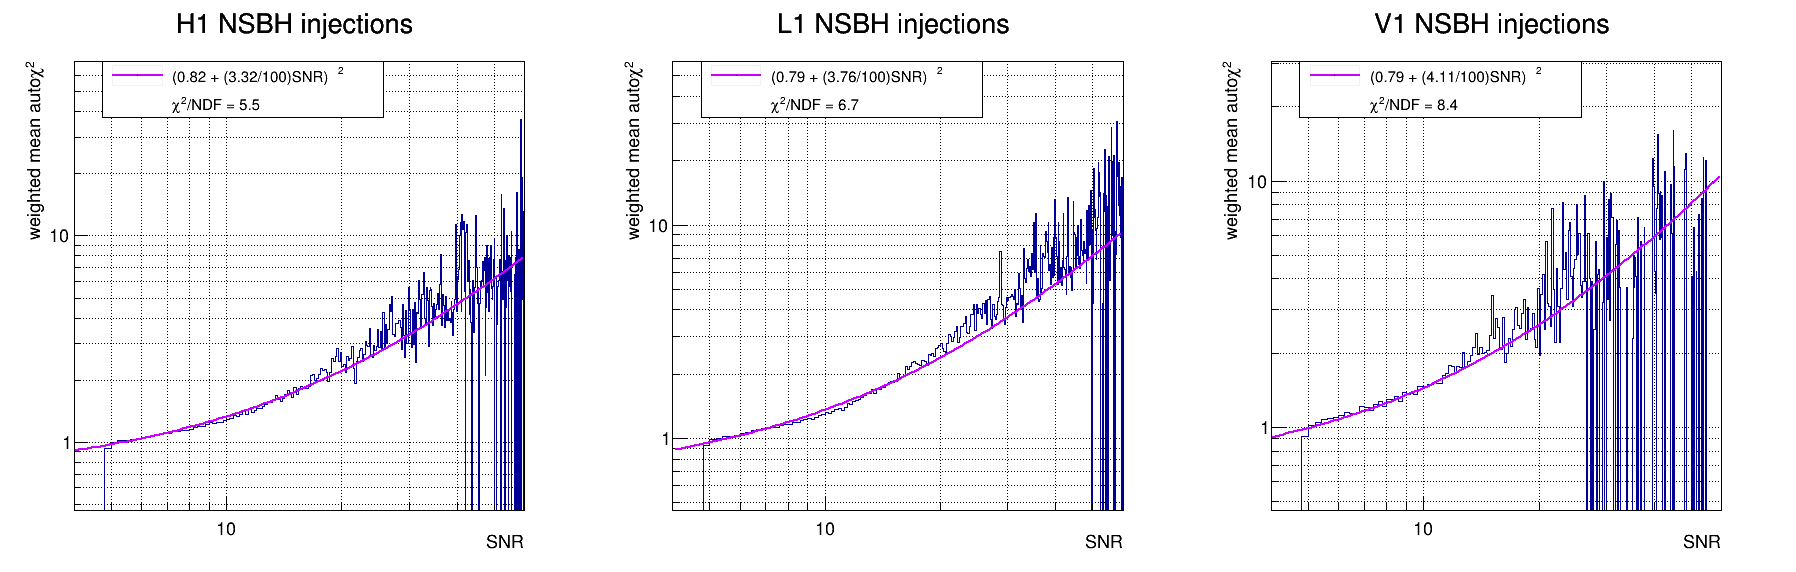
\includegraphics[width = \textwidth]{sectionImprovement/rwSNR/cProfile_NSBH.png}
  \end{minipage}
  \caption{Injections \achi vs SNR profile histograms. From top to bottom: BBH injections, BNS injections and NSBH injections.}
  \label{fig:fit_profile}
\end{figure}




%%%%%%%%%%%%%%%%%%%%%%%%%%%%%%%%%%%%%%%%%%%%%%%%%%%%%%%%%%%%%%%%%
%%%%%%%%%%%%%%%%%%%%%%%%%%%%%%%%%%%%%%%%%%%%%%%%%%%%%%%%%%%%%%%%%
%%%%%%%%%%%%%%%%%%%%%%%%%%%%%%%%%%%%%%%%%%%%%%%%%%%%%%%%%%%%%%%%%

\subsection{Mitigating the SNR dependence in the reweighting}
\label{sec:new_reweight}
We would like to  mitigate the SNR dependence of the reweighting induced by the SNR dependence of the $\achi$.
We tried to modify the reweighting formula \ref{eq:rwsnr} as follows:
%
\begin{equation}
\label{eq:new_rwsnr}
    \textrm{rwSNR} = \begin{cases}
    \textrm{SNR} &, \textrm{ if \achi} \leq \left(C+\epsilon\textrm{ SNR}\right)^2.\\
    \textrm{SNR}\left( \frac{ A+\left[\frac{\achi}{\left(C+\epsilon\textrm{ SNR}\right)^2}\right]^\alpha }{A+1} \right)^{-\frac{1}{\beta}} &, \textrm{ otherwise}.
  \end{cases}
\end{equation}
%
The idea here is to start reweighting at higher \achi for higher SNRs, the modified numerator ensures the continuity of the weight applied at 1.
This is actually identical to defining a new \achi such that
%
\begin{equation}
\label{eq:new_achi2}
    \achi' = \frac{\achi}{\left(C+\epsilon\textrm{ SNR}\right)^2}
\end{equation}
%
and we would have the following reweighting formula:
%
\begin{equation}
\label{eq:new_old_rwsnr}
    \textrm{rwSNR} = \begin{cases}
    \textrm{SNR}, & \textrm{if \achi}' \leq 1.\\
    \textrm{SNR} \times \left( \frac{ A+\left[\achi'\right]^\alpha }{ A+1 } \right)^{-\frac{1}{\beta}}, & \text{otherwise}.
  \end{cases}
\end{equation}
%
which is identical to equation \ref{eq:achi2} when switching $\achi \leftrightarrow \achi'$.
%
\begin{figure}[ht]
    \centering
    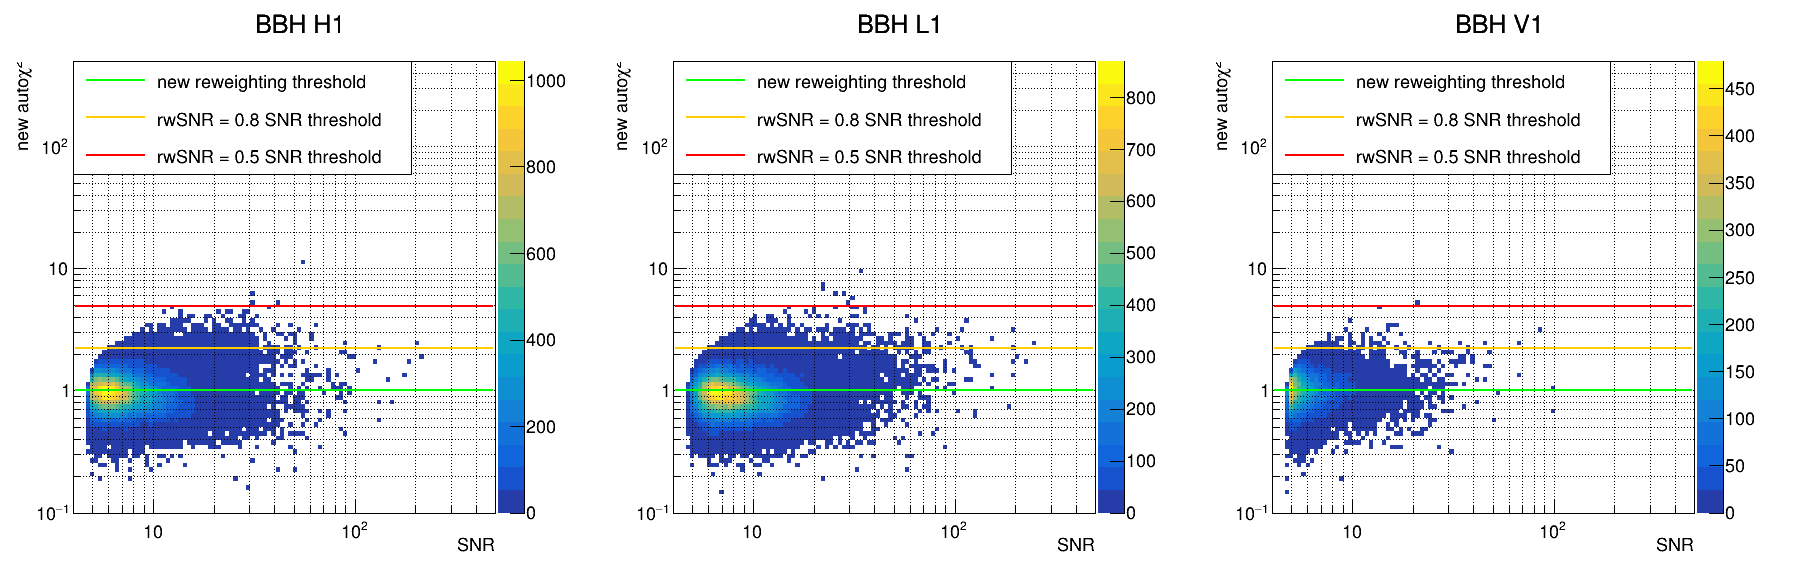
\includegraphics[width=\textwidth]{sectionImprovement/rwSNR/cSnrAchi2P.png}
    \caption{O3 BBH recovered injections: $\achi'$ (or new $\achi$) vs SNR for single detector triggers associated to coincidences.}
    \label{fig:new_achi2vsSNR}
\end{figure}
%

As the parameter values of the fits presented in the different plots in figure \ref{fig:fit_profile} seem to be uncorrelated with the detector and the type of source (as they should be), we decide to take the mean value over the detectors and sources: we therefore settle for $C=0.82$ and $\epsilon = 0.033$ .
Figure \ref{fig:new_achi2vsSNR} shows the distribution of O3 BBH injections in the $\achi'$ versus SNR plane.
The $\achi'$ works as intended with a much flatter distribution in SNR.
Figure \ref{fig:new_thresholds} shows the new thresholds for $\text{rwSNR} = 100\%/80\% \text{SNR}$ using the formula with the $\achi'$ \ref{eq:new_old_rwsnr}.
We were able to make an SNR-dependent reweighting that is less harsh at high SNR but we are now barely reweighting the background: almost all triggers keep more than 80\% of their SNR.

The next step of the study was to explore different values of the parameters with the $\achi'$.
The figure of merit of this analysis is the number of recovered injections at high SNR versus the number of background triggers.
But we also have to keep in mind that the efficiency of the search is computed using the global number of recovered injections, meaning that we do not want to lose (too many) injections at low SNR.
In an attempt to tune further the formula we explore higher values of the parameter $\alpha$ to give more weight to the term containing the $\achi'$.
After several attempts we choose a value of $\alpha = 12$ instead of 5.
Figure \ref{fig:all_thresh} shows the same thresholds as figure \ref{fig:new_thresholds} but with $\alpha = 12$ for injections and background.
Detection thresholds are also plotted.
\begin{figure}[ht]
  \centering
  \begin{minipage}{0.45\linewidth}
    \centering
    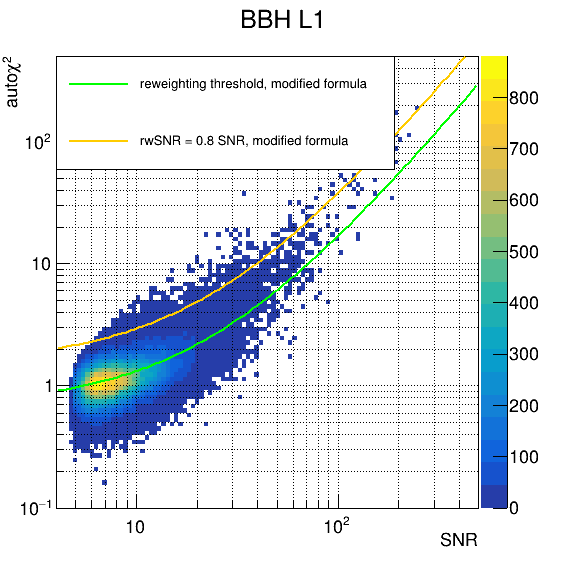
\includegraphics[width=\textwidth]{sectionImprovement/rwSNR/cSnrAchi2_new_L1.png}
  \end{minipage}
  \hfill
  %% 
  \begin{minipage}{0.45\linewidth}
    \centering
    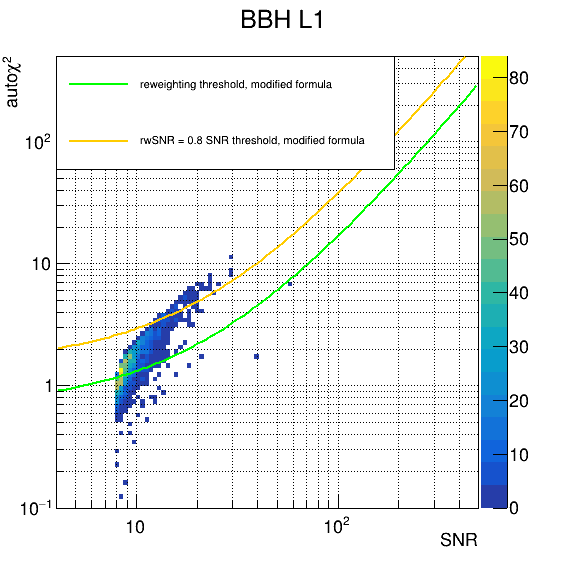
\includegraphics[width=\textwidth]{sectionImprovement/rwSNR/cSnrAchi2_singles_new_L1.png}
  \end{minipage}
  \hfill
  \caption{\achi vs SNR. Left: single detector triggers associated to coincidences for O3 BBH recovered injections. Right: O3 BBH background single detector triggers. The reweighting threshold and rwSNR = 80\% SNR obtained using the modified formula \ref{eq:new_rwsnr} with $\alpha = 5$ are also plotted.}
  \label{fig:new_thresholds}
\end{figure}

We show also in figures \ref{fig:new_rwsnr_inj} and \ref{fig:new_rwsnr_singles}, for injections and background respectively for the full O3 run, the rwSNR distribution obtained using the formula \ref{eq:new_rwsnr} with $C=0.82$, $\epsilon=0.033$ and $\alpha=12$ (mind the rwSNR threshold value that is different for background and injections in these plots).
As intended we now recover more injections at high SNR and the background remains globally unchanged but on the downside we lose some injections at low rwSNR and we actually lose more of them than we gain at high rwSNR, meaning that the efficiency of the search is actually lowered.
Other modifications of the reweighting formula were considered to try to improve the rwSNR.
They did not allow for any significant improvement of the \achi but they were documented with their pros and cons \cite{technote_rwsnr}.

In figure \ref{fig:new_rwsnr_singles} in L1, we note the presence of 3 triggers with a modified rwSNR larger than 30.
All 3 of those are caused either by scattered light in the detector or glitches and are associated to the exact same short (template duration=0.62), very asymmetric (mass1=193.011, mass2=2.02908) template.
A scan centered on the time of one of them is shown in figure \ref{fig:trig30}.
It is therefore safe to consider that the presence of these 3 events at high modified rwSNR does not contradict the work presented here.
This issue of "noisy templates" was investigated in section \ref{section:selection}.




%%



%%
\begin{figure}
  \centering
  \begin{minipage}{0.45\linewidth}
    \centering
    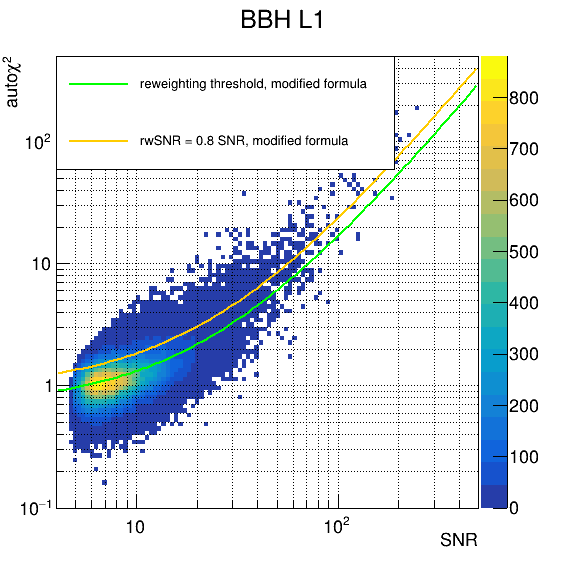
\includegraphics[width=\linewidth]{sectionImprovement/rwSNR/cSnrAchi2_new_L1_a12.png}
    %\caption{O3 BBH injections, $\alpha = 12$: green, purple and blue threshold are the same as figure \ref{fig:new_thresholds}. The yellow and red lines show the threshold for the rwSNR to pass the pipeline cuts with the old and modified formula respectively.}
    %\label{fig:all_thresh_inj}
  \end{minipage}
  \hfill
  %%%%
  \begin{minipage}{0.45\linewidth}
    \centering
    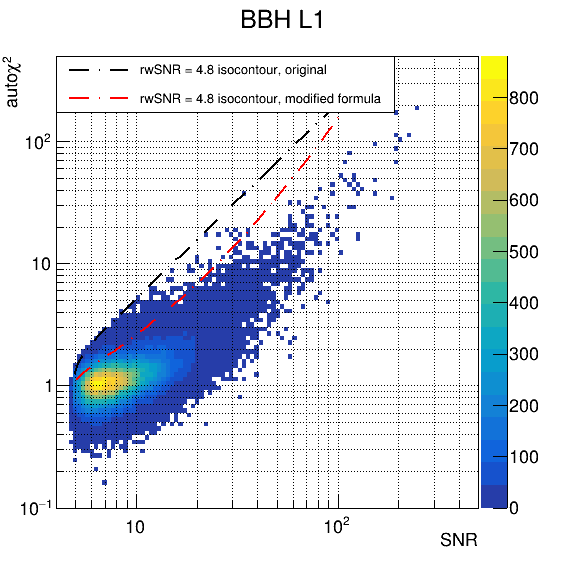
\includegraphics[width=\linewidth]{sectionImprovement/rwSNR/cSnrAchi2_new2_L1_a12.png}
    %\caption{O3 BBH injections, $\alpha = 12$: green, purple and blue threshold are the same as figure \ref{fig:new_thresholds}. The yellow and red lines show the threshold for the rwSNR to pass the pipeline cuts with the old and modified formula respectively.\textcolor{red}{modifier legende + coller aux plots singles en 2x2}}
    %\label{fig:all_thresh_inj}
  \end{minipage}
  \hfill
  %%%%
  \begin{minipage}{0.45\linewidth}
    \centering
    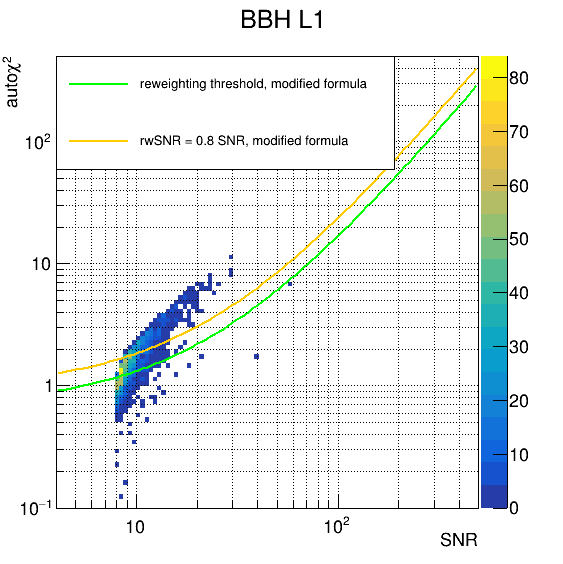
\includegraphics[width=\linewidth]{sectionImprovement/rwSNR/cSnrAchi2_singles_new_L1_a12.png}
    %\caption{O3 BBH injections, $\alpha = 12$: green, purple and blue threshold are the same as figure \ref{fig:new_thresholds}. The yellow and red lines show the threshold for the rwSNR to pass the pipeline cuts with the old and modified formula respectively.}
    %\label{fig:all_thresh_inj}
  \end{minipage}
  \hfill
  %%%%
  \begin{minipage}{0.45\linewidth}
    \centering
    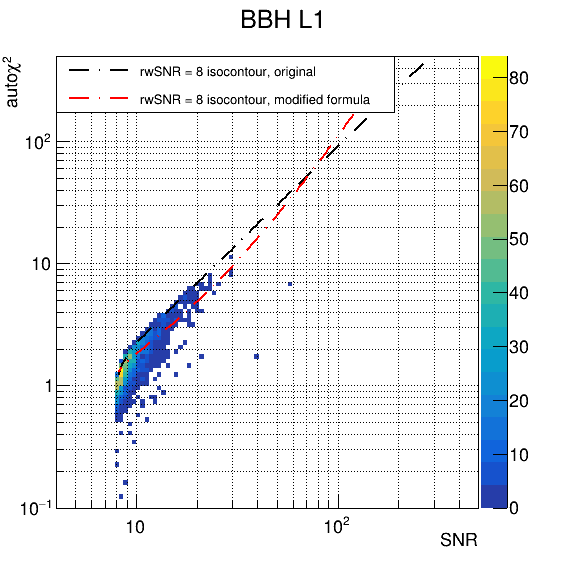
\includegraphics[width=\linewidth]{sectionImprovement/rwSNR/cSnrAchi2_singles_new2_L1_a12.png}
    %\caption{O3 BBH injections, $\alpha = 12$: green, purple and blue threshold are the same as figure \ref{fig:new_thresholds}. The yellow and red lines show the threshold for the rwSNR to pass the pipeline cuts with the old and modified formula respectively.\textcolor{red}{modifier legende + coller aux plots singles en 2x2}}
    %\label{fig:all_thresh_inj}
  \end{minipage}
  \caption{Top plots: O3 BBH injections \achi vs SNR dsitribution with rwSNR thresholds as a fraction of the SNR (left) and detection threshold (right) using $\alpha = 12$ in formula \ref{eq:new_rwsnr}.
  Bottom plots: same plots for O3 BBH background single detector triggers.}
  \label{fig:all_thresh}
\end{figure}
%%
%%
\begin{figure}[ht]
    \centering
    \includegraphics[width=\textwidth]{sectionImprovement/rwSNR/cRwSnr_a12.png}
    \caption{O3 BBH injections: comparison of the rwSNR distribution using the modified reweighting formula versus the original one.}
    \label{fig:new_rwsnr_inj}
\end{figure}
%%
%%
\begin{figure}[ht]
    \centering
    \includegraphics[width=\textwidth]{sectionImprovement/rwSNR/cRwSnr_singles_a12.png}
    \caption{O3 BBH background single detector triggers: comparison of the rwSNR distribution using the \achi2' and $\alpha=12$ versus the original one.}
    \label{fig:new_rwsnr_singles}
\end{figure}
%%
%%
%%
%%
\begin{figure}[ht]
  \centering
  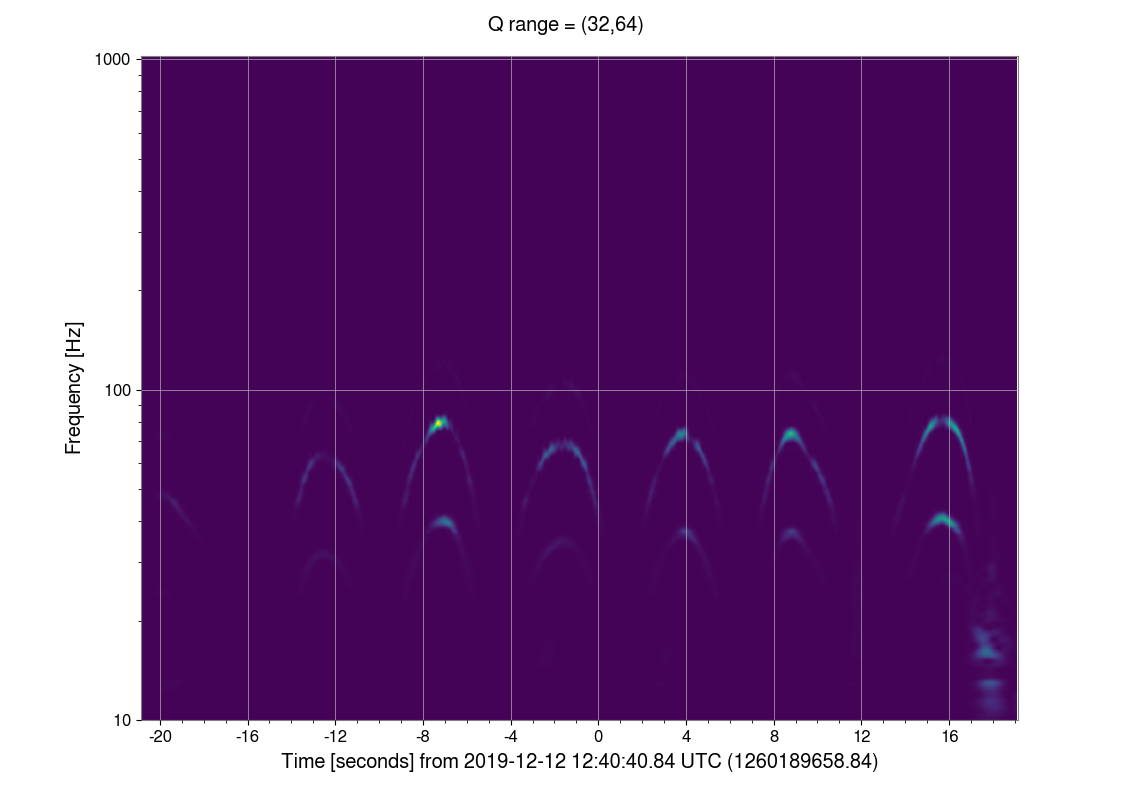
\includegraphics[width=0.5\linewidth]{sectionImprovement/rwSNR/1260189658.84_1.png}
  \caption{Trigger in L1 at GPS=1260189658.84 with modified rwSNR=59.28 .}
  \label{fig:trig30}
\end{figure}



